\mathchardef\mhyphen="2D % Define a "math hyphen"

\section{Methodology}
\label{sec:methodology}

In this paper, we use the IP ID side channel (Section~\ref{sec:ipidchannel})
to determine whether a particular online host blocks traffic using one
or more known blacklists. In brief, we begin by identifying hosts that are
suitable for this technique. We refer to such hosts as
\emph{reflectors}. Then we randomly sample a set of IP addresses
from IP blacklists that could be used to block traffic. We call
such IP addresses \emph{blacklist IPs}. Then we measure if
each reflector blocks packets whose source addresses are blacklist
IPs. If one reflector blocks all IP addresses we sampled
from one particular blacklist, then it is probably using that blacklist.

In this section, we first describe how the technique works at a
high-level (Section~\ref{sec:meththeory}). Then we detail
our method for identifying proper {\reflectors} for the
measurement (Section~\ref{sec:methrefl}), how we choose target blacklists to test (Section~\ref{sec:methblkl}), and how to sample IP addresses from each
blacklist (Section~\ref{sec:methtarg}). In Section~\ref{sec:methtrain}, we
explain the experiment design in detail and how it works in
real world scenarios. Section~\ref{sec:methvalid} further describes the steps
we take to sanity check, and in Section~\ref{sec:ethics} we discuss the
ethical considerations of our methodology.

\subsection{Technique Overview}
\label{sec:meththeory}

To measure if one {\reflector} is blocking one particular IP from a blacklist,
we send a train of packets (in our approach we use SYN-ACK packets)
from our measurement machine to the {\reflector}. The packet train consists
of packets whose source address is the blacklist IP (spoofed),
bracketed by packets whose source address is our measurement machine,
as illustrated in Figure~\ref{fig:coreidea}. If a firewall in the
reflector's network blocks packets from the blacklist IP, the
reflector will not receive packets with the blacklisted source address. In
this case, it will only receive packets with our measurement machine's source
address. On the other hand, if there is no firewall blocking such packets, the
reflector will receive the entire packet train.

%a variation of the Ensafi technique proposed for censorship
%measurement~\cite{ensafi2014detecting}.

\begin{figure}[t]
    \centering
    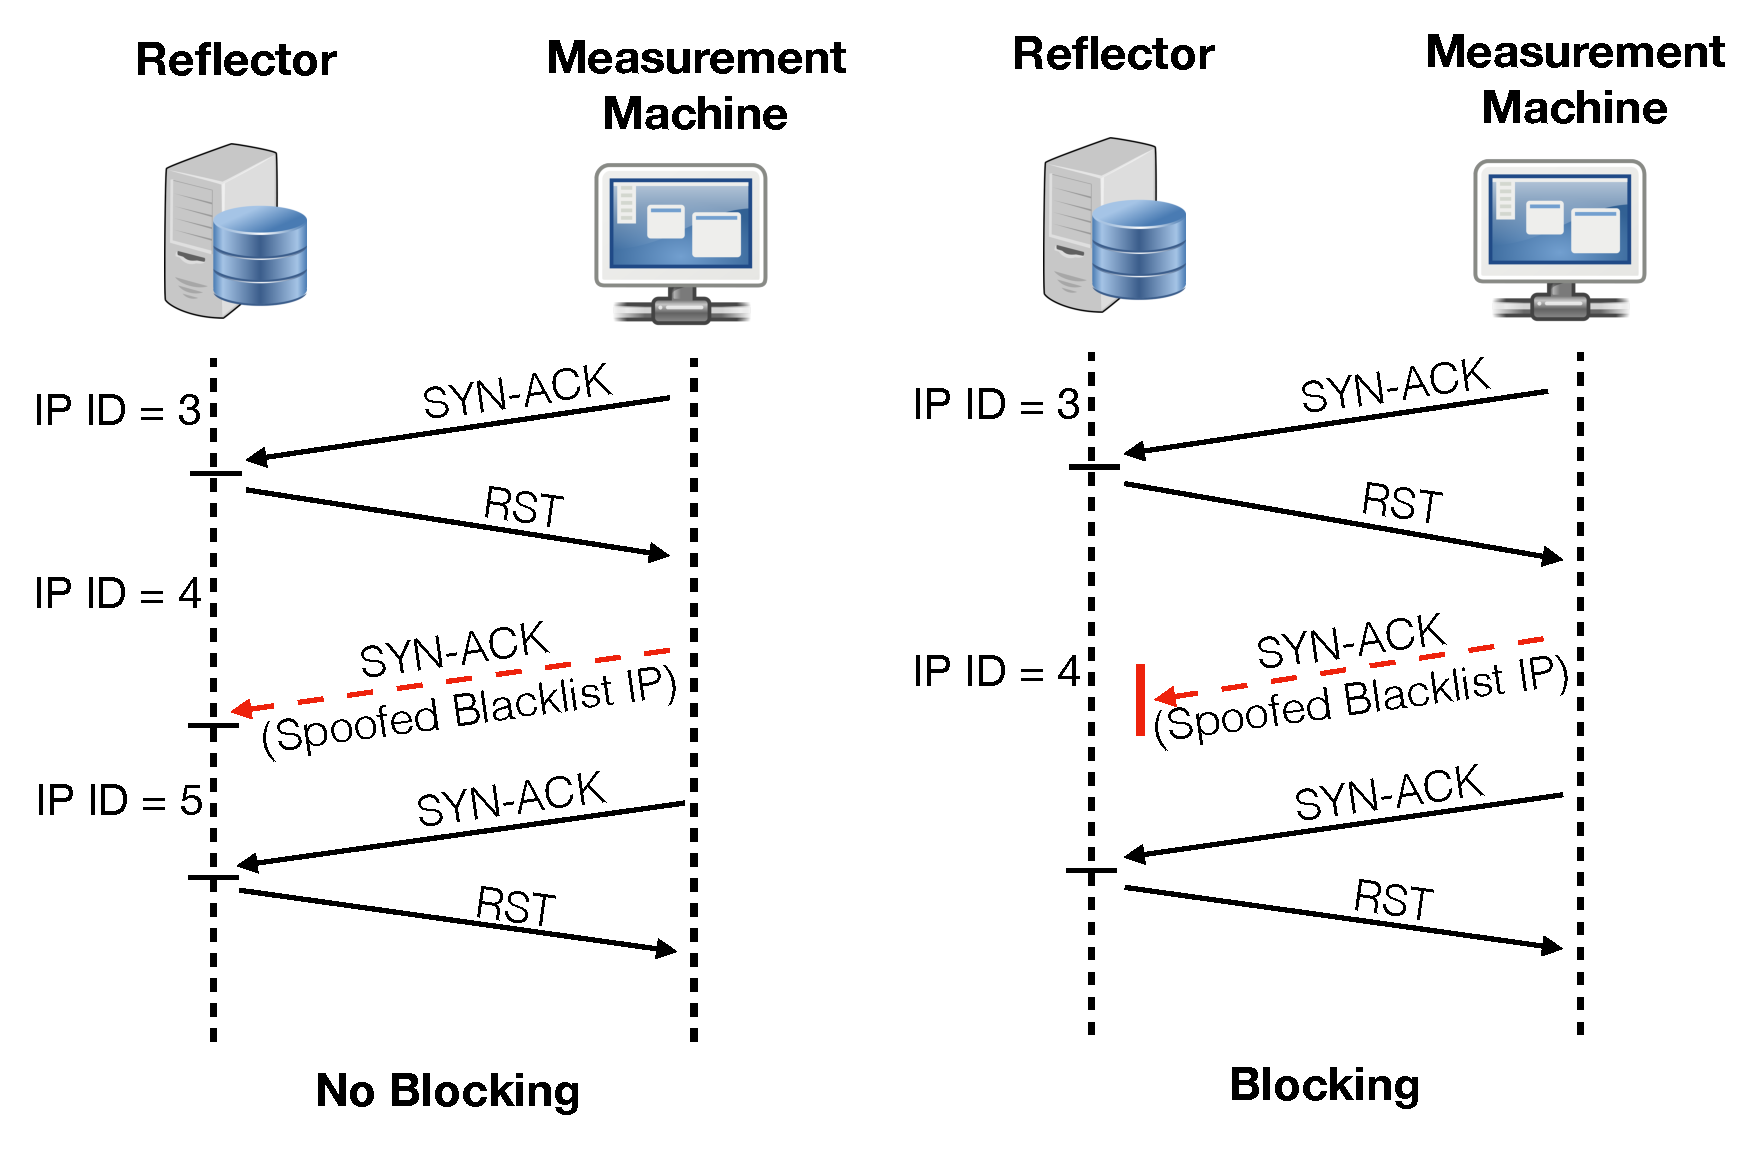
\includegraphics[width=0.98\columnwidth]{data_usage/images/cropped_method_protocol_v2.pdf}
    \caption{The basic method to detect network packet blocking using the IP ID side channel.}
    \label{fig:coreidea}
\end{figure}

In an ideal world, where there is no packet loss during transmission
and no extra traffic on the {\reflector}, we would see a clear difference
in the IP IDs we get from the responses between the two different scenarios.
In particular, we expect the {\reflector} to send a RST response for
each SYN-ACK packet we send, and we will receive the responses for
the SYN-ACK with our measurement machine's source address. The IP IDs of these
received RST packets will reflect the number of
packets sent by the reflector. If the reflector did not receive the SYN-ACK
packets with the blacklist IP as source addresses( because they were blocked by a
firewall), the IP ID sequence in the RST responses will be an
increasing sequence without gaps (the ``Blocking'' case in Figure~\ref{fig:coreidea}).
On the other hand, if the reflector did
receive the SYN-ACK packets with the blacklist IP, it would have sent
a RST packet in response to each such packet, incrementing the IP ID counter
each time. While we will not see the RST packets sent to the blacklist
IP, we \emph{will} observe the increments in the IP ID sequence.
More specifically, we would see a gap in the IP ID sequence of packets received
by our measurement machine (the ``No Blocking'' case in
Figure~\ref{fig:coreidea}).
These two cases, illustrated in Figure~\ref{fig:coreidea}, allow us to
determine whether a particular blacklist IP is blocked by some network
device, such as a firewall, somewhere between the measurement host and
the reflector. When there is no blocking in place (left), the measurement
machine will see an IP ID gap in two RST responses: the second IP ID will
increase by two. Whereas if there is network blocking (right), then the
two IP IDs will not have a gap: the second IP ID will only increase by
one.
%and this gap should equal the number of RST
%packets sent to the blacklisted addresses, which, in turn, should equal the
%number of SYN-ACK packets received by the reflected with the blacklisted
%address.

This measurement technique is inspired by the method proposed in previous
work~\cite{ensafi2014detecting, pearce2017augur}.  However, to make it work for
our objective we need to handle a few more important issues, as we will
see in the rest of this section.

\subsection{Compare with Previous Method}

At a high level, the objective of the measurement is to determine, from a third
point, if a {\reflector} blocks a blacklist IP. The blocking behavior that we
want to measure is \textit{inbound blocking} -- that is the incoming traffic
is blocked and as a result traffic does not reach the intended host. A
typical example is a network firewall, where it can stop certain network
packets from reaching hosts behind the firewall. Here we abstract the
{\reflector} as $Host_A$, blacklist IP as $Host_B$, and the problem is to
detect the connectivity between two hosts on the Internet.

%Another type of blocking is %\textit{outbound blocking}, where the outgoing
%traffic to a ``blocked host'' from a host within the network is blocked. %A
%typical example is network censorship. Our measurement in this paper only
%focuses on inbound blocking, %and we will explain more about this in the
%following sections.

\begin{figure}[t]
\centering
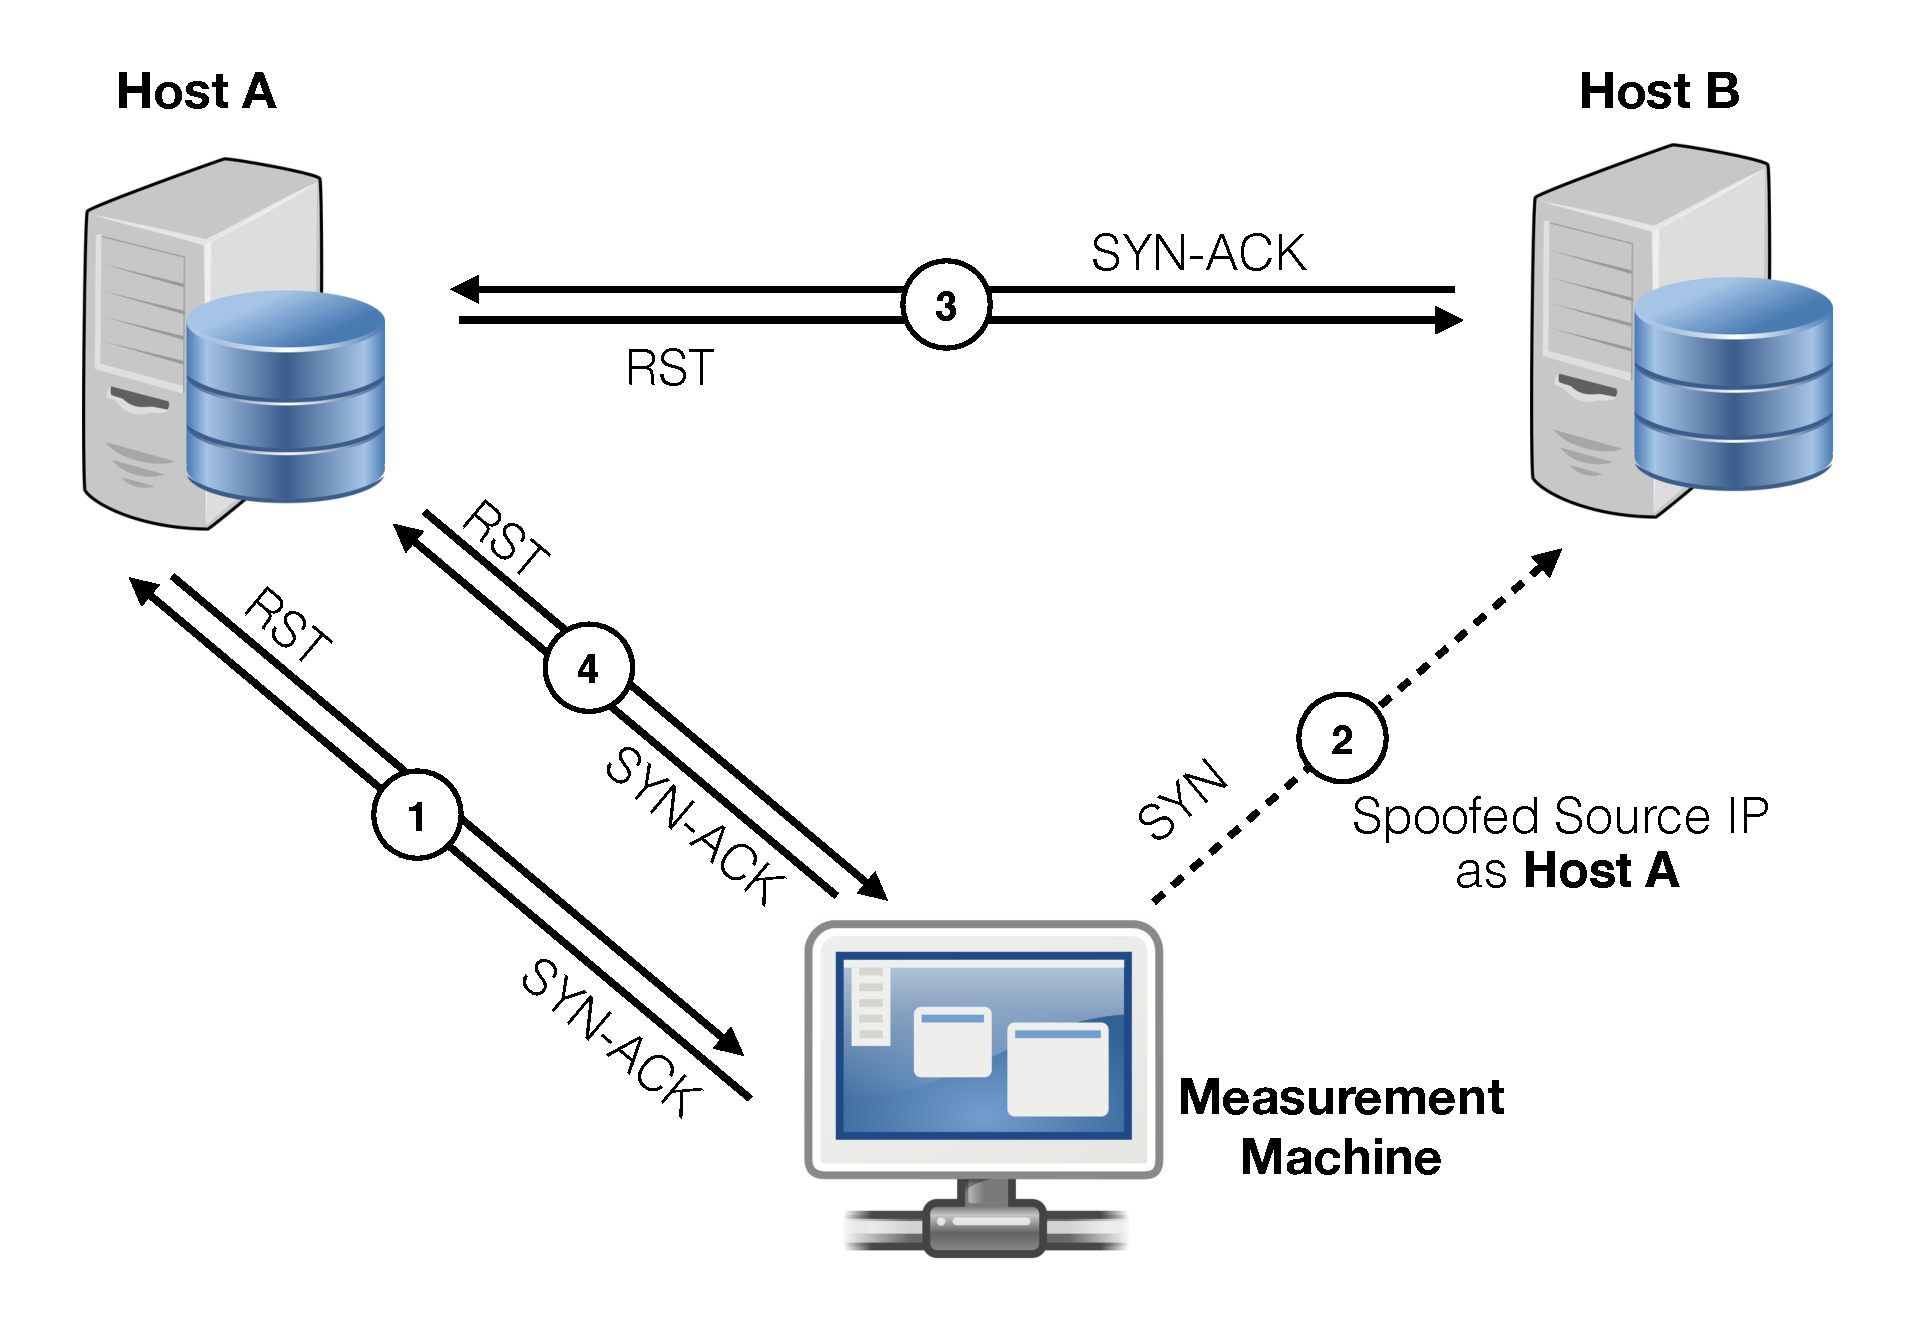
\includegraphics[width=0.8\columnwidth]{data_usage/images/croped_method_old.pdf}
\caption{Measurement method used in previous work.}
\label{fig:old_method}
\end{figure}

In previous works~\cite{pearce2017augur, ensafi2014detecting}, to measure
the connectivity between two hosts from a third party, they send spoofed packets
to impersonate one of the hosts. This methodology -- one we refer
to as the \textit{triangle measurement} takes advantage of the TCP 3-way
handshake protocol, as shown in Figure~\ref{fig:old_method}.

The measurement machine first sends a probe to the $Host_A$, in this case a TCP
SYN-ACK packet. $Host_A$ responds with a RST packet since it received a SYN-ACK
without the preceding SYN packet. Thus, the measurement machine gets the
first IP ID $IP\mhyphen ID_1$ from the RST packet (corresponds to Step 1 in
the figure). Next, the measurement machine sends a spoofed TCP SYN packet to
$Host_B$, with source IP address set to the IP address of $Host_A$ (Step 2).
$Host_B$ then sends a responding SYN-ACK packet to $Host_A$, which causes $Host_A$
to respond with a RST packet (Step 3), and increment its IP ID counter by 1.
Finally, the measurement machine probe $Host_A$ again and get the second IP ID
$IP\mhyphen ID_2$ (Step 4).

Now we can infer whether $Host_A$ is inbound blocking traffic from $Host_B$ by
observing the difference between $IP\mhyphen ID_1$ and $IP\mhyphen ID_2$.
Assuming there is no packet loss, and that $Host_A$ does not have any extra
traffic besides our measurement traffic, then
$IP\mhyphen ID_2 = IP\mhyphen ID_1 + 2$ implies there is no inbound blocking,
since it indicates that $Host_A$ received both packets in step 3 and step 4,
while $IP\mhyphen ID_2 = IP\mhyphen ID_1 + 1$ means there is blocking.

Previous work chose this ``triangle measurement'' because it ensures that in
step 3, the packets from $Host_B$ will go through the same routes as the
traffic originated from $Host_B$. So from $Host_A$'s perspective, it can not
identify that the traffic from $Host_B$ are spoofed. However, in this schema,
one hard requirement is that $Host_B$ needs to be active and responding to TCP
SYN probe. This is not an issue for censorship measurement, as $Host_B$ in this
case are popular sites (Google, Facebook, Twitter etc.) that guaranteed will
respond to SYN probe.

However, in our case, we need to measure whether $Host_A$ is blocking traffic
from a blacklist IP($Host_B$). But there is no guarantee that these IP
addresses are active and thus may not respond to our SYN probe. In fact, we
found that the percentage of responding IPs in a blacklist can be as low as less
than 20\%. This dramatically reduces the candidate IPs we can sample from a
blacklist to test, especially for small blacklists that only have a few hundred
IPs. Furthermore, there are many other additional constraints when shortlisting
IPs for measurement from a blacklist.
The requirement that blacklist IPs respond to SYN probe does not work for our
use case. 
%\textcolor{red}{Explain the choice for only inbound blocking}

In order to get around this limitation we adjust the measurement methodology.
In this new methodology, the measurement machine directly sends spoofed
packets to the target host, as shown in Figure~\ref{fig:new_method}. In
this case, the measurement machine first probes $Host_A$ to get the first IP ID
$IP\mhyphen ID_1$, then it sends a spoofed packet, with source IP set to
$Host_B$(Blacklist IP), directly to $Host_A$. Finally, it sends a second probe
to $Host_A$ and get the second IP ID $IP\mhyphen ID_2$. Now we can use the same
logic as before to infer whether $Host_A$ is inbound blocking $Host_B$. In this
approach, we do not require $Host_B$ to be actively responding SYN packets, any
IP address can be used here to conduct the test. The drawback is that the
spoofed packets now at times go through a different route versus the packets
originated from $Host_B$. Some network that implement spoofed packet
detection~\cite{ferguson2000rfc2827} could drop our spoofed packets, giving us
a false signal of inbound blocking. Therefore, when selecting hosts we conduct
extensive tests to weed out hosts that have such detection logic in place. We
find that not a lot of target hosts have such detection logic. We will talk in
detail about host selection in the follow sections.

%Therefore, we modified the measurement so that the measurement machine  directly
%send spoofed packets to host A, as shown in Figure~\ref{fig:new_method}. In
%this case, the measurement machine first probes host A to get the first IP ID
%\texttt{IP\_ID\_1}, then it sends a spoofed packet, with source IP as host B,
%directly to A. Finally, it sends a second probe to host A and get the second
%IP ID \texttt{IP\_ID\_2}. Now we can use the same logic as before to infer
%whether host A is inbound blocking host B. In this approach, we do not
%require host B to be actively responding SYN packets, any IP address can be
%used here to conduct the test. The drawback now is that the spoofed packets
%will likely go through a different route versus the packets originated from
%host B. Some network that implemented spoofed packet detection~\cite{ferguson2000rfc2827}
%could drop our spoofed packets, giving us a false
%signal of inbound blocking. Therefore, when selecting hosts for the
%measurement, we conduct extensive tests to make sure the hosts do not have
%such detection logic in place. Our experiment also shows that not a lot of
%hosts have such detection logic. We will talk in detail about host selection
%in Section~\ref{sec:requirement_host}.

\begin{figure}[t]
\centering
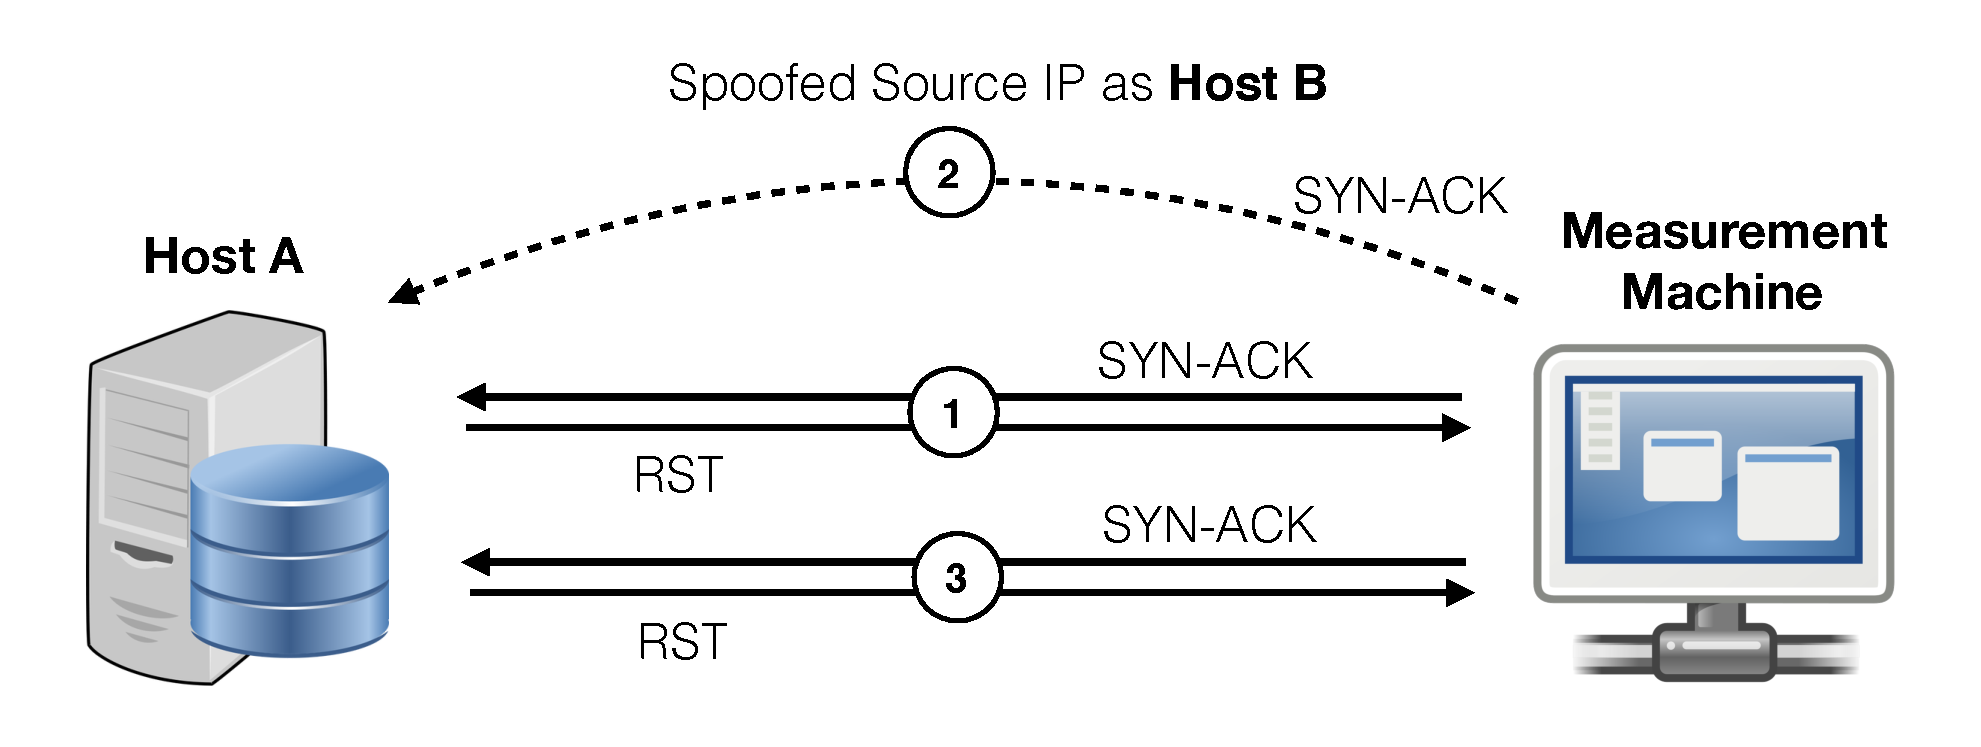
\includegraphics[width=0.8\columnwidth]{data_usage/images/croped_method_new.pdf}
\caption{Measurement method used in this work.}
\label{fig:new_method}
\end{figure}

\subsection{Finding Suitable Reflectors}
\label{sec:methrefl}

At a high level, our methodology relies on being able to infer blocking
using the IP ID side channel. Keeping that in mind, listed below is the
criteria we look for when scanning the Internet to search for suitable
reflectors.

\begin{itemize}
    \item \textbf{RST packet generation:}
    The {\reflectors} must reply with a RST packet to a TCP SYN-ACK packet without an
    established connection. Some hosts drop incoming SYN-ACK packets if there
    is no corresponding SYN packet. These hosts are not suitable for our
    measurement methodology. We choose SYN-ACK packets instead of SYN because
    it does not create an intermediate state on the {\reflectors} and
    connection is terminated in one go.

    \item \textbf{Shared monotonic increasing IP ID counter:}
    The IP ID counter in the {\reflector} needs to be globally shared, so all
    network traffic generated from the host will use the same counter for IP
    ID assigning. It also needs to be monotonically increasing, so we can
    observe the number of packets generated by the host between two measurements using
    the difference of IP IDs.
    %This is the side channel we discussed before and it is the pre-condition for
    %all of our measurement.
    \item \textbf{Low traffic:}
    Our technique requires the host to have low traffic volumes
    in general, since the technique depends on the fact
    that we can observe a clear difference in IP ID increases when sending
    spoofed packets. If there are always many other
    packets coming to the host, it would be infeasible to observe the IP ID
    changes triggered by our measurement packets.

    \item \textbf{No ingress filtering:}
    We send spoofed packets to {\reflectors} to infer traffic blocking.
    However, some network providers utilize ingress filtering techniques and
    drop packets once they detect the packets are not from the networks they
    claimed to originate. This would cause our spoofed packets being dropped
    and give us a false signal of traffic blocking.

    \item \textbf{No stateful firewall blocking:}
    Some networks deploy a stateful firewall that blocks access from a source IP
    after receiving too many repetitive packets. One example is to defend
    against SYN floods~\cite{lemon2002resisting}. While we try to keep the number
    of our measurement packets as low as possible, if our spoofed packets trigger such
    firewall rules and then we are blocked by the firewall, we will incorrectly
    conclude that the {\reflector} uses a blacklist to block that IP.
\end{itemize}

%The criteria laid out for selecting reflectors is fairly conservative since
%one of the major goals of this paper is to show that our methodology is
%reliably able to infer blacklist use. However, we expect a more lenient
%criteria for the reflectors with minor changes to our methodology to still work.
%Also, to avoid blocking due to censorship and other policy related blocking
%we focus on hosts in the United States.
We try to uncover how online hosts are using IP blacklists to
block traffic. But when we look at the problem on a global scale, there are
many policy related reasons why a host blocks network traffic,
such as censorship. These alternate sources of blocking could disrupt our
measurement, making it hard to distinguish the type of security-related blocking we target.
To simplify the problem, in this paper we focus on the hosts in
United States.


We find {\reflectors} in the United States with open ports using a snapshot
of Censys~\cite{censys} scanning data from November 8, 2019. We
then scan these 40 million hosts to identify the ones with the IP ID side channel. We send multiple probes to each host targeting an open port from different
source addresses, and then check IP IDs in the responses. In the case where hosts have
multiple open ports, we randomly select a port to send the probe.

To identify stateful firewalls, we send SYN-ACK packets to each {\reflector}
in two different patterns: 1 second per packet with 24 packets, and 5 packets
per second with 60 packets, which corresponds to the speed we probe
{\reflectors} during actually experiments (see the following section). We
repeat each experiment 6 times and discard the hosts that block us after the
experiment. To find the hosts with low extra traffic, we send 24 probes
to each host, 1 per second, and repeat the experiment 5 times at different
times of the day. We then collect the result and only select the hosts where
more than 30\% of their IP ID increases are equal to 1 per second --- that is,
the host did not receive any extra traffic besides our probes,
and all of the increases were smaller than 10 within a second.

Finally, we try to identify hosts experiencing ingress filtering. To
account for differences in ingress filtering that may possibly occur on
different network paths to the {\reflectors}, we acquired 7 vantage points around
the world to exercise different paths. %These vantage points are
%from the US west coast, east coast and midwest, and places in Asia, Europe,
%Australia and South America.
We then send spoofed packets from our measurement
machine to the {\reflectors} with spoofed source addresses corresponding to
the 7 vantage points, and later collect responses at each vantage point.
We only select the {\reflectors} that send responses to all 7
vantage points, meaning they did not drop spoofed packets on these network paths.

Eventually, we identified {\reflcount} IP addresses in US that meet our
requirements.\footnote{We
initially discovered more than 300K {\reflectors}, but during our
experiments some hosts became inactive. The number reported here is the
final number after we finished all our experiments.} For the purpose of this paper, here we treat each individual IP
address as a distinct {\reflector}. Detailed numbers are presented in
Table~\ref{tab:target-hosts}.

\begin{table}[t]
\centering
\caption{The number of {\reflectors} (IP addresses) identified in the United States, and the
corresponding count of /24 prefixes and Autonomous Systems.}
\begin{tabular}{l >{\hfill}p{4.5cm}}
 \toprule
 Category                    &  Count    \\
 \midrule
 \textbf{IP Addresses}       &  \reflcount  \\
 \textbf{/24 Count}          &  128,712  \\
 \textbf{Autonomous Systems} &  3,371    \\
%% \textbf{Organizations}      &  3,321    \\
 \bottomrule
\end{tabular}
%% and organizations (One organization can have multiple ASes)}
\label{tab:target-hosts}
\end{table}

\subsection{Choosing the Blacklists}
\label{sec:methblkl}
%By far we have demonstrated the methodology and the requirements for selecting
%measurement candidates. One question we have not addressed is what IP blacklists
%we choose to test against. Section~\ref{sec:methodology} described the criteria
%for sampling blacklist IPs from a given blacklist, but we still need to pick
%the blacklist in the first place.

\begin{table}[t]
\centering
\caption{Top {\blacklistnum} popular public IP blacklists.}
\begin{tabular}{l r}
 \toprule
\textbf{Blacklist}   & \quad\quad \textbf{Average Number of IPs} \\
 \midrule
 \textbf{\spamhausdrop}                 & $\sim$ 20,000,000       \\
    \multicolumn{2}{l}{    Spamhaus Don't Route Or Peer Lists}  \\
    %\hspace{0.2cm}    https://www.spamhaus.org/drop/drop.txt \\

 \textbf{\spamhausedrop}                &  $\sim$ 900,000          \\
    \multicolumn{2}{l}{    An extension of the Spamhaus DROP list} \\
    %\hspace{0.2cm}    https://www.spamhaus.org/drop/edrop.txt \\

 \textbf{\dshieldtop}                   &  5,120            \\
    \multicolumn{2}{l}{    DShield.org recommended top 20 /24s to block} \\
    %\hspace{0.2cm}    https://www.dshield.org/block.txt \\

%\textbf{\ciarmy}                       & 15,000            \\
    %\multicolumn{2}{l}{    Collective Intelligence Network Security(CINS) blacklist} \\
    %\hspace{0.2cm}    http://www.ciarmy.com/list/ci-badguys.txt \\

 \textbf{\etcompromised}                & $\sim$ 400               \\
    \multicolumn{2}{l}{    EmergingThreats.net recorded compromised hosts} \\
    %\multicolumn{2}{l}{\hspace{0.2cm} https://rules.emergingthreats.net/blockrules/compromised-ips.txt} \\

 \textbf{\snortfilter}                  & $\sim$ 1,500             \\
    \multicolumn{2}{l}{    labs.snort.org supplied IP blacklist}  \\
    %\hspace{0.2cm}    http://labs.snort.org/feeds/ip-filter.blf \\

 \textbf{\bdsatif}                      & $\sim$ 6,000             \\
    \multicolumn{2}{l}{    Binary Defense System ban list} \\
    %\hspace{0.2cm}    https://www.binarydefense.com/banlist.txt \\

 \textbf{\feodo}                        & $\sim$ 700              \\
    \multicolumn{2}{l}{    Abuse.ch Feodo tracking list}  \\
    %\hspace{0.2cm}    https://feodotracker.abuse.ch/downloads/ipblocklist.txt \\

 \textbf{\blocklistde}                  & $\sim$ 30,000           \\
    \multicolumn{2}{l}{    Blocklist.de blacklist IPs} \\
    %\hspace{0.2cm}    http://lists.blocklist.de/lists/all.txt\\

 \textbf{\ettor}                        & $\sim$ 6,000             \\
       \multicolumn{2}{l}{ IPs that belong to Tor network (not just exits node)}  \\
       %\multicolumn{2}{l}{\hspace{0.2cm}    https://rules.emergingthreats.net/blockrules/emerging-tor.rules} \\
 \bottomrule
\end{tabular}
\label{tab:target-blacklists}
\end{table}

We choose candidate blacklists from public IP blacklists since we
do not have access to commercial blacklists. In this work, we use the
FireHOL IP blacklist collection~\cite{firehol} which aggregates over 100 public IP
blacklists. However, we cannot reasonably test against all the blacklists and
so, for the purposes of this paper, we would like to select the most popular
public IP blacklists and then do a more detailed measurement of them.

For each of the public IP blacklists, we sample five IPs (using the criteria
in Section~\ref{sec:methtarg}) from each list and test how many {\reflectors}
block all sampled blacklist IPs in each blacklist (using the method in
Section~\ref{sec:methtrain}). With this experiment, we
generate a list of the most popular blacklists. Of course, five sample points
from one list is not a strong enough indicator to conclude whether a host is
using that blacklist or not. That said, the goal of this measurement is not to
identify the exact hosts that use each blacklist. Rather, it is
estimate how widely used these blacklists might be so that we can use them for more detailed measurements. We
repeat the measurement twice and select the top {\blacklistnum} popular
blacklists,\footnote{We initially selected 10 blacklists. However, one blacklist,
abuse.ch Ransomware List, was discontinued by the provider during our
experiments, and so we removed that blacklist from consideration.} as listed in
Table~\ref{tab:target-blacklists}.

Note, the {\ettor} is the combination of three Tor blacklists, as they mostly
have the same content. This is primarily done since the huge overlap between
the three lists means that we have very few blacklist IPs that meet our
exclusive criteria (see Section~\ref{sec:methtarg}). The {\ettor} essentially
includes IPs for all nodes in the Tor network, including entry nodes, so the
{\reflectors} who block IPs on this list can neither be accessed from Tor nor
use Tor services themselves.

\subsection{Sampling Blacklist IPs}
\label{sec:methtarg}
%\noteby{KL}{As sketched above, we should describe our selection criteria as
%    being (a) some blacklisted addresses that are unique to each blacklist, and
%    (b) some blacklisted addresses that are common to many lists. This allows us
%    to determine whether a specific blacklist is used, as well as to determine if
%    \emph{some} blocking is taking place, even if we cannot identify the specific
%    blacklist.}

For determining if a {\reflector} uses a particular IP blacklist, we use a
sample of IPs from the blacklist to test since it is infeasible for us to
test all blacklist IPs. Further, to obtain a definitive signal from our
measurement, we adhere to the following constraints when sampling blacklist
IPs:

\begin{itemize}
    \item \textbf{Exclusive:}
    A blacklist can share part of its contents with other blacklists. To
    reasonably infer whether a {\reflector} is using a specific blacklist, we
    need to test with the IPs that are unique to that blacklist --- IPs that are
    only in this blacklist, but no others.

    \item \textbf{Stable:}
    The IPs on a blacklist change over time. To reliably measure if a
    {\reflector} blocks IPs from a certain blacklist, we need the
    sampled IPs to stay in the blacklist throughout our measurement. We discard
    any measurements where the blacklist IP does not remain on the blacklist for
    the duration of the measurement.

    \item \textbf{Routable:}
    IP blacklists can contain unroutable IPs~\cite{li2019reading}. Sending
    packets with an unroutable source address results in a large portion of
    packets being dropped (which could potentially happen at the end ISP or the
    transient link). Packet drops due to unroutable IPs would create noise in our measurement.
    Therefore, when sampling IPs from blacklists we ensure that the
    IPs are routable.

    \item \textbf{Geo-location diversified:}
    Besides blacklisting, another common reason for a host to block certain
    traffic is geo-blocking, where a host blocks all traffic coming from a certain
    country or a certain region. To minimize the effect of geo-blocking, we
    prioritize IPs that are from the United States when sampling IPs. The assumption is that a
    host in the US will not block traffic from its own country. For IPs from other
    countries, we try to increase the diversity of IP locations, making sure
    these IP are not concentrated in a few countries when possible.

    \item \textbf{Not from the hosts' network (AS disjoint):}
    We observed many networks drop spoofed packets when the spoofed source addresses are
    within their own network. So when selecting IPs, we make sure that these IPs
    are not from the same ASes as one of our {\reflectors}.

\end{itemize}

To obtain ``exclusive'' IPs from a blacklist, we would potentially need an
``oracle'' that includes all IP blacklists, which is impractical. In this work,
we use the public IP blacklists collected by FireHOL, as mentioned earlier, to calculate the
exclusive part of each target blacklist. For ``stable'' IPs, we
collect all the target blacklists hourly, and ensure the sampled IPs are in
the blacklist through the duration of the experiment. To satisfy the
``routable'' requirement, we use the daily RouteView data~\cite{Routeview}
to identify BGP routable IPs. As for geo-location diversity, we use
Netacuity~\cite{netacuity} to make sure for each experiment the sampled IPs
cover as many different countries as the data allows.
